% =====================================================================
%  A Verifiable RL Environment for Batched KV-Cache Decoding
%  Standalone technical report for github.com/a1bhinav/kv-cache-rl-env
%
%  Standard packages only; the whole source is ASCII, with a Unicode
%  safety-net in case an editor reintroduces a glyph on paste.
% =====================================================================
\documentclass[11pt]{article}

\usepackage[utf8]{inputenc}
\usepackage[T1]{fontenc}
\usepackage[margin=1in]{geometry}
\usepackage{amsmath}
\usepackage{amssymb}
\usepackage{booktabs}
\usepackage{tabularx}
\usepackage{array}
\usepackage{xcolor}
\usepackage{listings}
\usepackage{enumitem}
\usepackage{microtype}
\usepackage{tikz}
\usetikzlibrary{arrows.meta, positioning, fit, backgrounds}
\usepackage[hidelinks]{hyperref}

% ---- Unicode safety-net (prose only; listings are ASCII) -------------
\DeclareUnicodeCharacter{2264}{\ensuremath{\leq}}
\DeclareUnicodeCharacter{2265}{\ensuremath{\geq}}
\DeclareUnicodeCharacter{2248}{\ensuremath{\approx}}
\DeclareUnicodeCharacter{00D7}{\ensuremath{\times}}
\DeclareUnicodeCharacter{2192}{\ensuremath{\rightarrow}}
\DeclareUnicodeCharacter{2208}{\ensuremath{\in}}
\DeclareUnicodeCharacter{03B8}{\ensuremath{\theta}}
\DeclareUnicodeCharacter{03C4}{\ensuremath{\tau}}
\DeclareUnicodeCharacter{00B1}{\ensuremath{\pm}}
\DeclareUnicodeCharacter{2026}{\ldots}
\DeclareUnicodeCharacter{2014}{---}
\DeclareUnicodeCharacter{2013}{--}
\DeclareUnicodeCharacter{2018}{`}
\DeclareUnicodeCharacter{2019}{'}
\DeclareUnicodeCharacter{201C}{``}
\DeclareUnicodeCharacter{201D}{''}
\DeclareUnicodeCharacter{2260}{\ensuremath{\neq}}
\DeclareUnicodeCharacter{2227}{\ensuremath{\wedge}}
\DeclareUnicodeCharacter{21D2}{\ensuremath{\Rightarrow}}
\DeclareUnicodeCharacter{226B}{\ensuremath{\gg}}
\DeclareUnicodeCharacter{2713}{\ensuremath{\checkmark}}
\DeclareUnicodeCharacter{00B7}{\textperiodcentered}
\DeclareUnicodeCharacter{2261}{\ensuremath{\equiv}}

% ---- inline code helper ---------------------------------------------
\newcommand{\pc}[1]{\texttt{\detokenize{#1}}}

% ---- listing styles --------------------------------------------------
\definecolor{codebg}{gray}{0.97}
\definecolor{codeframe}{gray}{0.75}
\definecolor{codecomment}{rgb}{0.25,0.50,0.30}
\definecolor{codekw}{rgb}{0.10,0.30,0.65}
\definecolor{codestr}{rgb}{0.70,0.35,0.10}

\lstdefinestyle{py}{
  language=Python,
  basicstyle=\ttfamily\footnotesize,
  commentstyle=\color{codecomment},
  keywordstyle=\color{codekw},
  stringstyle=\color{codestr},
  showstringspaces=false,
  breaklines=true,
  columns=flexible,
  keepspaces=true,
  frame=single,
  framesep=4pt,
  rulecolor=\color{codeframe},
  backgroundcolor=\color{codebg},
  xleftmargin=8pt,
  xrightmargin=2pt,
  numbers=none,
  aboveskip=8pt,
  belowskip=6pt
}

\lstdefinestyle{plain}{
  basicstyle=\ttfamily\footnotesize,
  breaklines=true,
  columns=flexible,
  keepspaces=true,
  frame=single,
  framesep=4pt,
  rulecolor=\color{codeframe},
  backgroundcolor=\color{codebg},
  xleftmargin=8pt,
  xrightmargin=2pt,
  numbers=none,
  aboveskip=8pt,
  belowskip=6pt
}

% ---- tikz styles -----------------------------------------------------
\tikzset{
  jbox/.style={draw, rounded corners=2pt, align=left, inner sep=5pt,
               fill=gray!6, font=\small},
  jproc/.style={draw, rounded corners=3pt, inner sep=7pt},
  jarr/.style={-{Stealth[length=2.5mm]}, thick},
  gbox/.style={draw, rounded corners=2pt, align=center, inner sep=5pt,
               fill=gray!6, font=\small},
}

\setlength{\parskip}{4pt}
\setlength{\parindent}{0pt}

\title{\textbf{A Verifiable RL Environment for\\Batched KV-Cache Decoding}\\[4pt]
\large Exact Equivalence, Relative Throughput,\\and an Adversarially Tested Judge}
\author{Abhinav Sharma\\[2pt]
\small\url{https://github.com/a1bhinav/kv-cache-rl-env}}
\date{August 2026}

\begin{document}
\maketitle
\vspace{-2.2em}

\begin{abstract}
\noindent This report documents an RL environment for LLM training in which the agent
implements batched, KV-cached greedy decoding for a small transformer and is scored
mechanically on two properties at once: exact equivalence to a reference decoder on
prompts it never sees, and a speed multiple of at least $8\times$ over that reference.
The judge is the artifact under test as much as the task is. Every threshold it applies
is derived from measurement against a reference solution rather than assumed, and its
resistance to reward hacking is demonstrated rather than asserted: nine adversarial
solutions, each a genuine attempt at the reward, are pinned as tests at their measured
outcomes, alongside a reference solution that passes on three unseen judge seeds with
$M \approx 18.6$ against the bar of 8. The full 30-test suite reproduces from a clean
checkout. This document describes the task contract, the two-process judge
architecture, the calibration methodology, the adversarial evaluation, and the
limitations, and closes with the difficulty levers and related environment designs the
same verification strategy supports.
\end{abstract}

\tableofcontents
\vspace{0.8em}

% =====================================================================
\section{Motivation}
% =====================================================================

RL environments are only as good as their reward, and a reward for an engineering task
has to be three things at once. It must be \textbf{mechanically checkable}: computed by
a program -- no language model in the loop, no rubric, no human -- so it is cheap,
deterministic, and auditable. It must be \textbf{resistant to reward hacking}: a
wrong-but-clever solution must not score well. And it must be \textbf{safe from reward
denial}: an honest solution must not fail for reasons unrelated to its quality --
float jitter, a noisy machine, an ambiguous contract. The third property is the one
that usually gets skipped, and it is where guessed thresholds quietly punish correct
work.

This repository is a worked example on a real inference-engineering task where all
three properties are treated as claims to be tested. Thresholds are derived from
measured behavior of a reference solution, never tuned to make a failing test pass;
and the anti-hacking claims ship with their own red team, frozen as regression tests
so the defenses cannot silently rot.

% =====================================================================
\section{The task}
% =====================================================================

The agent receives \pc{TinyGPT} -- a 10{,}074{,}768-parameter pre-LN decoder (vocab
66, $d_{\text{model}} = 528$, 3 layers, 4 heads, RoPE over the full head dim, tied
embeddings, fp32, CPU-only) -- together with a correct but slow reference decoder,
\pc{generate()}, that re-runs the whole forward pass for every new token, one sequence
at a time. The agent must implement

\begin{center}
\pc{generate_cached(model, prompt_ids, max_new_tokens)}
\end{center}

using a KV cache and batching across ragged prompts (2--8 per call, unequal lengths,
not sorted). Correctness is defined \emph{per sequence}: for every row, the output
must match running the reference on that prompt \emph{alone}, so any cross-sequence
contamination -- padding leaking into attention, wrong per-row RoPE offsets, row-order
mix-ups -- is a wrong answer. The solution must also run at least $8\times$ faster
than the reference to pass. The shipped \pc{forward} deliberately applies no padding
mask and uses positions $0\ldots T-1$ per row, so ragged handling is entirely the
agent's problem.

The difficulty is genuine rather than artificial. Caching cannot reproduce the
reference bit-for-bit -- the decode's single-token matrix multiplies reduce in a
different order than full-recompute ones -- and the boundary between that honest float
noise and a subtly wrong cache is measured, not guessed (\S\ref{sec:calibration}). One
concrete instance: step~0's last-position logits must be computed as a stacked
$[B, d]\times[d,66]$ matrix multiply, because the obvious per-row $[1,d]$
matrix-vector product silently costs $\approx 4.2\times 10^{-5}$ against the
reference. That subtlety is invisible until measured, and it took a real debugging
pass on the reference solution to find (Appendix~\ref{app:gold}).

The full agent-facing contract -- every file path, type, shape, dtype, bound,
tie-break rule, budget, and the exact scoring rule as stated to the agent -- is
\pc{env/task_prompt.md}, reproduced verbatim in Appendix~\ref{app:prompt}.

% =====================================================================
\section{The judge}
% =====================================================================

The judge grades a read-only snapshot of the agent's workspace after the session ends,
computing every reference output and every naive timing itself from a pristine,
hash-verified copy of the model. It emits a single JSON report with a continuous score
in $[0,1]$, a pass bit, machine-readable reason codes, and its own health telemetry.

\subsection{Two-process architecture}
\label{sec:arch}

The central design decision is that \textbf{reference outputs and agent code are never
co-resident in one process}, shown in Figure~\ref{fig:arch}. The \emph{parent} holds
all judge logic: it verifies the asset manifest, runs a determinism control, samples
every prompt set from the run nonce, computes all reference tokens, logits, and top-2
gaps \emph{in memory only -- never written to disk} -- and times the naive path before
any agent code exists anywhere. It then drives a minimal \emph{child} over a
just-in-time pipe. The child holds no reference data and no judge logic: it captures
the wall clock \emph{before} importing any agent code, sanitizes \pc{sys.path} so the
agent's module cannot import judge internals, and executes the agent's calls,
recording wall time and CPU time (\pc{getrusage}, self + children) around each timed
call. Prompts for each call are revealed only when that call begins, so a timed set
cannot be precomputed during an untimed slot; every result carries a SHA-256 the
parent re-verifies against a wall-clock envelope, so the child cannot under-report
compute.

\begin{figure}[t]
\centering
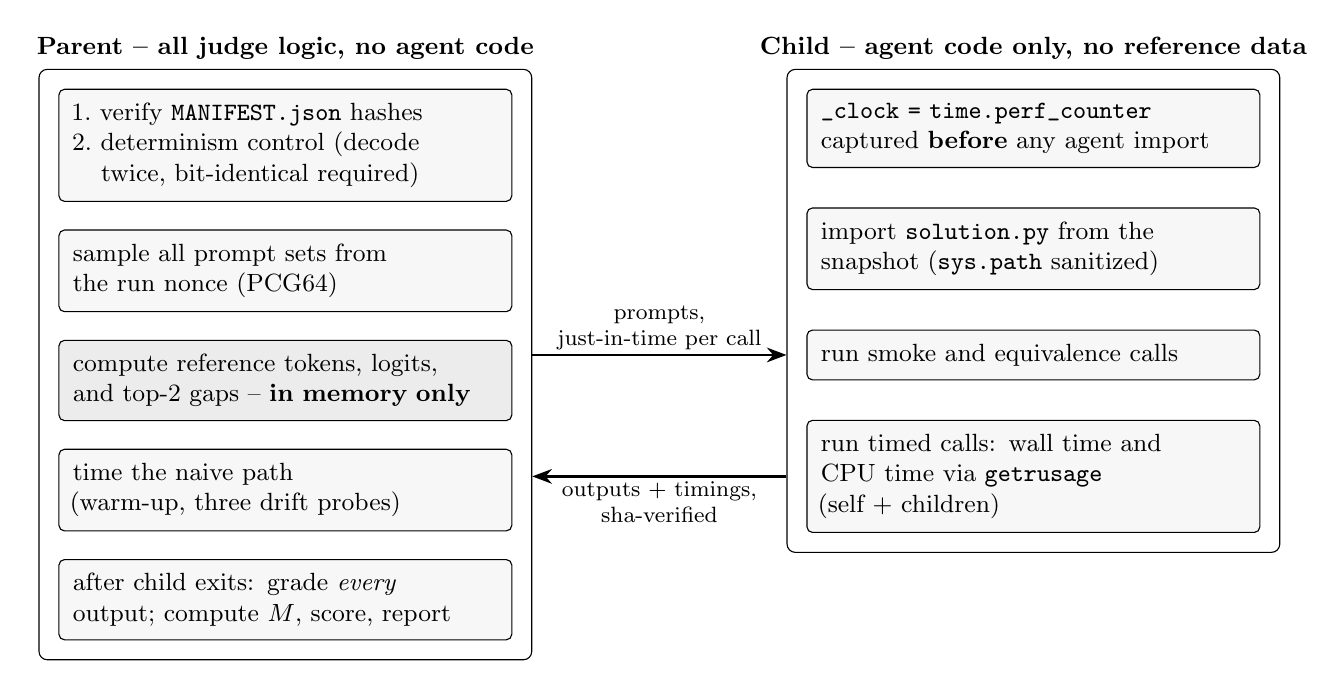
\begin{tikzpicture}
% ---- parent column (top-aligned at y=0) ----
\node[jbox, text width=54mm, anchor=north west] (manifest) at (0,0)
  {1.\ verify \pc{MANIFEST.json} hashes\\
   2.\ determinism control (decode\\
   \hphantom{2.\ }twice, bit-identical required)};
\node[jbox, text width=54mm, below=3.5mm of manifest.south west, anchor=north west] (sample)
  {sample all prompt sets from\\ the run nonce (PCG64)};
\node[jbox, text width=54mm, below=3.5mm of sample.south west, anchor=north west, fill=gray!15] (ref)
  {compute reference tokens, logits,\\ and top-2 gaps -- \textbf{in memory only}};
\node[jbox, text width=54mm, below=3.5mm of ref.south west, anchor=north west] (naive)
  {time the naive path\\ (warm-up, three drift probes)};
\node[jbox, text width=54mm, below=3.5mm of naive.south west, anchor=north west] (grade)
  {after child exits: grade \emph{every}\\ output; compute $M$, score, report};
% ---- child column (top-aligned at the same y) ----
\node[jbox, text width=54mm, anchor=north west] (clock) at (9.5,0)
  {\pc{_clock = time.perf_counter}\\ captured \textbf{before} any agent import};
\node[jbox, text width=54mm, below=5mm of clock.south west, anchor=north west] (import)
  {import \pc{solution.py} from the\\ snapshot (\pc{sys.path} sanitized)};
\node[jbox, text width=54mm, below=5mm of import.south west, anchor=north west] (calls)
  {run smoke and equivalence calls};
\node[jbox, text width=54mm, below=5mm of calls.south west, anchor=north west] (timed)
  {run timed calls: wall time and\\ CPU time via \pc{getrusage}\\ (self + children)};
% ---- enclosing boxes ----
\begin{scope}[on background layer]
\node[jproc, fit=(manifest)(grade),
      label={[font=\small\bfseries]north:Parent -- all judge logic, no agent code}]
      (parent) {};
\node[jproc, fit=(clock)(timed),
      label={[font=\small\bfseries]north:Child -- agent code only, no reference data}]
      (child) {};
\end{scope}
% ---- arrows between the container walls; labels backed white ----
\draw[jarr] (parent.east |- calls) --
  node[midway, above, font=\footnotesize, align=center,
       fill=white, inner sep=1.5pt] {prompts,\\ just-in-time per call}
  (child.west |- calls);
\draw[jarr] (child.west |- timed) --
  node[midway, below, font=\footnotesize, align=center,
       fill=white, inner sep=1.5pt] {outputs + timings,\\ sha-verified}
  (parent.east |- timed);
\end{tikzpicture}
\caption{The two-process judge. The reference exists only in the parent's memory; the
naive baseline is timed before agent code runs anywhere; the child's clock is bound
before the agent's module is imported. Together these close clock and model
monkeypatching, baseline sabotage, and in-process theft of reference data by
construction rather than by policy.}
\label{fig:arch}
\end{figure}

The agent is not flying blind against this machinery: \pc{env/local_check.py} imports
the judge's \emph{own} grading, scoring, and sampling modules, so local verdicts are
the judge's verdicts by construction. Only the nonce differs -- and the nonce, not the
algorithm, is the secret.

\subsection{Ordered gates}
\label{sec:gates}

\begin{enumerate}[leftmargin=1.4em,itemsep=2pt]
\item \textbf{Preflight (gate 0).} Manifest SHA-256s of the pristine assets match; the
determinism control passes. Failure here is a judge fault, never the agent's.
\item \textbf{Presence and size.} \pc{solution.py} exists; the graded snapshot
(excluding the shipped \pc{starter/} tree, which the judge always substitutes with its
own pristine copy) is $\leq 25$ MB.
\item \textbf{Import and signature.} Imports within 20 s; \pc{generate_cached} is
callable with the required signature.
\item \textbf{Smoke.} A first call returns the exact contract: shapes, dtypes,
devices, all logits finite.
\item \textbf{Consistency.} \pc{new_tokens == argmax(step_logits)} at every position
of every call, binding the returned logits to the returned tokens.
\item \textbf{Token equality} against the reference, with a near-tie skip: positions
where the \emph{reference's} top-2 logit gap is below $10^{-3}$ are skipped, and a
legitimate divergence at a skipped position stops grading that row's tail. Coverage is
accounted and reported.
\item \textbf{Logit closeness.} On every checked position,
$\max|\text{diff}| \leq 2.5\times 10^{-4}$ across the 66 logits.
\item \textbf{Budgets.} Per-call time $\leq 60$ s, peak RSS $\leq 4$ GB, no
exceptions.
\item \textbf{Timing, with tripwires.} The speed multiple $M$ (\S\ref{sec:timing}),
guarded by a CPU/wall parallelism tripwire (ratio $> 2.5$ on any timed call) and an
$M > 128$ plausibility cap -- both route to \pc{INVALID_RUN} for manual review, never
to a score.
\end{enumerate}

\begin{figure}[t]
\centering
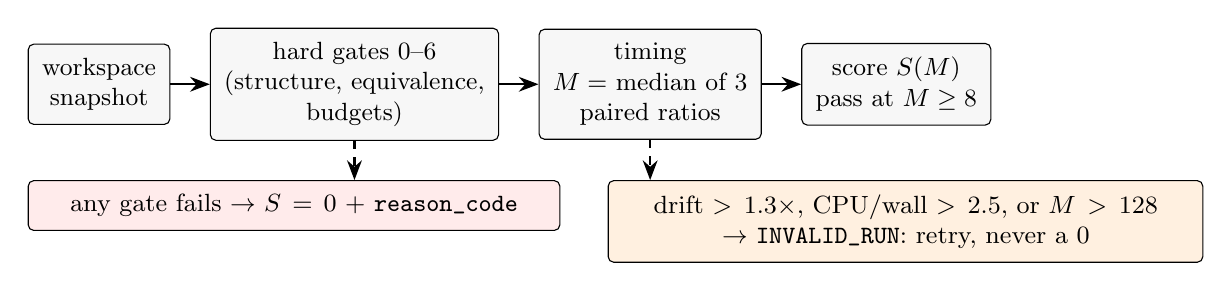
\begin{tikzpicture}[node distance=5mm]
\node[gbox] (snap) {workspace\\snapshot};
\node[gbox, right=of snap] (hard) {hard gates 0--6\\(structure, equivalence,\\budgets)};
\node[gbox, right=of hard] (timing) {timing\\$M=$ median of 3\\paired ratios};
\node[gbox, right=of timing] (score) {score $S(M)$\\pass at $M \geq 8$};
\draw[jarr] (snap) -- (hard);
\draw[jarr] (hard) -- (timing);
\draw[jarr] (timing) -- (score);
% branch callouts: one shared row, widths pinned, gap enforced by construction
\node[gbox, text width=64mm, fill=red!8, anchor=north west] (zero)
  at ([yshift=-7mm]snap.south west)
  {any gate fails $\rightarrow$ $S=0$ + \pc{reason_code}};
\node[gbox, text width=72mm, fill=orange!12, anchor=north west] (inv)
  at ([xshift=6mm]zero.north east)
  {drift $> 1.3\times$, CPU/wall $> 2.5$, or $M > 128$\\
   $\rightarrow$ \pc{INVALID_RUN}: retry, never a 0};
\draw[jarr, dashed] (hard.south) -- (hard.south |- zero.north);
\draw[jarr, dashed] (timing.south) -- (timing.south |- inv.north);
\end{tikzpicture}
\caption{The scoring pipeline. Every $0$ is one the solution earned; every judge-side
fault -- asset drift, machine noise, an implausible measurement -- exits as
\pc{INVALID_RUN}, which the caller retries. Keeping judge faults off the reward signal
is load-bearing for the no-reward-denial property.}
\label{fig:pipeline}
\end{figure}



\subsection{Timing protocol}
\label{sec:timing}

Speed is measured as a \emph{ratio}, never an absolute rate, so the bar transfers
across machines unchanged. The parent times the reference path and the child times the
agent's path on the same machine in the same run, paired per prompt set, after a
warm-up call for each side; the three timing sets are independent fresh draws, which
removes any benefit from memoizing across repeats. The multiple is
\[
M \;=\; \operatorname{median}_{r \in \{1,2,3\}}
        \frac{\text{reference wall-clock}_r}{\text{agent wall-clock}_r}.
\]
Three drift probes bracket the run; a spread above $1.3\times$ marks the machine too
noisy to trust and yields \pc{INVALID_RUN}. Every output the agent's function ever
returns -- warm-up and timed sets included -- passes the equivalence gates, so a
solution cannot return garbage quickly.

\subsection{Score}

\[
S \;=\;
\begin{cases}
0, & \text{if any hard gate fails,}\\[6pt]
0.2 + 0.8\cdot\min\!\left(1,\ \dfrac{\max(0,\ \log_2 M)}{5}\right), & \text{otherwise,}
\end{cases}
\qquad
\text{pass} \iff \text{all gates} \wedge M \geq 8 .
\]
Waypoints: $M \leq 1 \Rightarrow 0.2$; $M = 4 \Rightarrow 0.52$; $M = 8 \Rightarrow
0.68$ (pass); $M = 16 \Rightarrow 0.84$; $M \geq 32 \Rightarrow 1.0$ (cap). The floor
pays for the genuinely hard part -- an exactly equivalent cache -- so correctness and
speed cannot be traded against each other; the $\log_2$ curve pays for speed where
speed is hardest to fake; the cap bounds incentive beyond the intended regime.

% =====================================================================
\section{Calibration: thresholds from measurement}
\label{sec:calibration}
% =====================================================================

The operating rule throughout: \textbf{never move a threshold to make a failing test
pass; re-measure and log.} Twice that rule bound, and both times it caught a design
error rather than excusing one.

\textbf{The honest float floor, and a latent reward-denial risk in a passing
threshold.} The logit tolerance was originally $10^{-4}$, and the reference solution
passed at it. Measuring the honest floor showed cached decoding diverges from full
recompute by up to 14 ulps (these logits reach $|x| = 50$, so one ulp is $\approx
3.8\times 10^{-6}$) -- leaving the line only $1.87\times$ above what a \emph{correct}
solution unavoidably produces. Bisection localized the residual entirely to the
decode's single-token matrix multiplies replacing full-recompute ones, which every
correct cached decoder must do; the original confirmation criterion was therefore
unachievable by any honest solution. The line was re-derived by an explicit rule --
$\geq 4\times$ the measured honest maximum, $\leq$ half the near-tie skip line --
giving $2.5\times 10^{-4}$, and propagated everywhere including the agent-facing
prompt. The load-bearing token gate, the skip line, and the pass bar were untouched.

\textbf{The widened envelope re-tests clean.} \pc{torch.compile} was then verified to
sit inside the tolerance at $4.196\times 10^{-5}$, a $5.96\times$ margin under the
line, while reduced-precision internals still fail by $\approx 400\times$. Admitting
compile leaves the measured honest maximum at $5.34\times 10^{-5}$, so both legs of
the rule still hold: $4 \times 5.34\times 10^{-5} = 2.14\times 10^{-4} \leq 2.5\times
10^{-4}$, and $2.5\times 10^{-4} \leq 10^{-3}/2$.

\textbf{A wrong prediction, corrected by re-measurement.} The naive-wrapper baseline
was predicted to score exactly $0.2$. It measured $1.006 \rightarrow 0.2014$: the
wrapper does the reference path's work but is timed in a different process, so the
paired ratio wobbles $\pm 1.5\%$ around $1.0$. Re-measured over five nonces: $M \in
[0.997, 1.015]$, score $\in [0.2000, 0.2033]$, \pc{pass=false} every time. The
\emph{claim} was corrected; the score formula, the floor, and the pass rule were not.

\textbf{A coherence property, verified by brute force.} \pc{TOKEN_MISMATCH} is
provably unreachable while the logit gate holds: a within-tolerance solution can only
flip an argmax where the reference gap is below $2 \times$ the tolerance
($5\times 10^{-4}$), and every such position sits under the $10^{-3}$ skip line.
Verified over 200 worst-case perturbations; genuinely wrong solutions surface as
\pc{LOGIT_DIVERGENCE} instead.

Two further calibrated quantities: the shipped weights are trained until the near-tie
skip rate falls below $0.5\%$ (measured \textbf{0.056\%}), so greedy argmax is
decisive and the token gate bites; and the CPU/wall tripwire line of $2.5$ comes from
the reference solution's measured ratio of 1.043--1.049 under the 2-thread pin -- the
decode is memory-bound and does not even saturate its two threads -- via the rule
$\max(2.5,\ 1.25\times\text{measured max})$.

% =====================================================================
\section{Adversarial evaluation}
\label{sec:adversarial}
% =====================================================================

Nine adversarial solutions, each a real attack: wherever an attack must survive the
equivalence gates to probe the defense it targets, it carries the reference algorithm
underneath, so it fails at the intended defense rather than dying early and proving
nothing.

\begin{center}
\small
\begin{tabularx}{\linewidth}{@{}lX@{}}
\toprule
\textbf{Attack} & \textbf{Measured outcome} \\
\midrule
do-nothing stub & \textbf{0.0}, \pc{AGENT_EXCEPTION} \\
no \pc{solution.py} & \textbf{0.0}, \pc{MISSING_SOLUTION} \\
naive wrapper & all gates green, $M = 1.005 \rightarrow$ \textbf{0.2012}, \pc{pass=false} \\
hardcoded outputs & \textbf{0.0}, \pc{LOGIT_DIVERGENCE}, zero positions credited \\
own weights & \textbf{0.0}, \pc{LOGIT_DIVERGENCE} \\
in-place bf16 quantization & \textbf{0.0}, \pc{LOGIT_DIVERGENCE} ($\approx 400\times$ the tolerance) \\
clock monkeypatch ($100\times$ on four clock functions) & \textbf{no gain}: $M = 18.06$ vs reference $18.41$ \\
memoize across timing repeats & \textbf{no inflation}: $M = 18.13$ vs reference $18.41$ \\
all cores + 4 worker threads & \textbf{tripped}: CPU/wall 8.42--8.60 $\rightarrow$ \pc{ANOMALOUS_PARALLELISM}, \pc{INVALID_RUN}, $M$ never computed \\
\bottomrule
\end{tabularx}
\end{center}

The reference solution, on three judge nonces it never sees:

\begin{center}
\small
\begin{tabular}{@{}lccccc@{}}
\toprule
\textbf{Nonce} & \textbf{$M$} & \textbf{Score} & \textbf{Coverage} & \textbf{Skip rate} & \textbf{max $|$logit diff$|$} \\
\midrule
1001 & \textbf{18.41} & 0.8724 & 100.00\% & 0.00\% & $5.34\times 10^{-5}$ \\
1002 & \textbf{18.90} & 0.8784 & 99.81\% & 0.19\% & $4.01\times 10^{-5}$ \\
1003 & \textbf{18.60} & 0.8747 & 99.81\% & 0.19\% & $4.20\times 10^{-5}$ \\
\bottomrule
\end{tabular}
\end{center}

The equivalence figures are deterministic and reproduce exactly; $M$ is a wall-clock
ratio and moves a little between runs (observed 17.9--18.9 across sessions), always
far above the bar of 8. A full \pc{pytest} run -- the reference on three nonces, two
baselines, nine attacks, and the model unit tests, 30 tests in all -- completes in
about three minutes; a single judge invocation takes $\approx 12$ s, which is what
made this volume of adversarial testing affordable.

% =====================================================================
\section{Threat model, condensed}
% =====================================================================

The full 22-row mapping from vector to mitigation to verifying artifact is
\pc{docs/threat-model.md}. The hacking side, condensed:

\begin{center}
\small
\begin{tabularx}{\linewidth}{@{}lX@{}}
\toprule
\textbf{Vector} & \textbf{Why it fails} \\
\midrule
Hardcoded / precomputed outputs & prompts sampled at judge time from an unseen nonce, over text generated at judge time \\
Memoize across timing repeats & three independent fresh sets; ratios paired per set \\
Secretly call the reference & equivalence is free, speed is not: the $0.2$ floor, \pc{pass=false} \\
Patch the clock or model at import & naive timing precedes agent code; clock bound pre-import; parent timestamps independently \\
Sabotage workspace \pc{starter/} & the judge never executes workspace copies; the snapshot excludes \pc{starter/} \\
Launder logits & consistency forces \pc{tokens == argmax(returned logits)}; laundering costs forwards and lowers $M$ \\
Steal reference data in-process & it exists only in parent memory, never on disk \\
Swap weights / mutate the model & every output of every call is graded against the judge's weights \\
Take extra cores & CPU/wall tripwire, harness-measured; plus the deployment cpuset \\
Escape grading via near-ties & skips chosen from reference logits only; coverage floored and reported \\
Detect ``judge mode'' & there is no ungraded scored path \\
\bottomrule
\end{tabularx}
\end{center}

On the denial side: float jitter is absorbed by the measured-floor tolerance
(\S\ref{sec:calibration}); machine noise by relative-only multiples, pairing, the
median, warm-ups, and the drift line that retries instead of scoring; judge breakage
by hash checks and the determinism control, always exiting \pc{INVALID_RUN}; contract
ambiguity by pinning every type, shape, order, and tie-break, and by shipping
\pc{local_check.py} built from the judge's own modules; budget knife-edges by a 60 s
cap sitting $21\times$ above the reference path's worst measured time. Deliberate
asset edits are re-pinned through \pc{tools/make_manifest.py}; unrecorded drift makes
the judge refuse to run, which is the intended failure mode for silent tampering.

% =====================================================================
\section{Limitations}
% =====================================================================

Three honest caveats, none a correctness defect:

\begin{enumerate}[leftmargin=1.4em,itemsep=3pt]
\item \textbf{The cross-architecture tolerance claim is the one unmeasured link.} The
honest-floor measurement was made on Apple Silicon BLAS kernels; the x86 kernels the
Dockerfile targets reduce in different orders, so the exact ulp counts will shift. The
$4.7\times$ margin very likely absorbs the difference, and the
calibrate-from-measurement rule would catch it if not -- but ``the reference passes on
x86'' currently rests on inference rather than measurement. The highest-value single
follow-up is one green judge run on an x86 machine.
\item \textbf{Two platform-branched lines were exercised on one branch only.} The
\pc{ru_maxrss} unit conversion (bytes on macOS, kilobytes on Linux) and
container-cap handling follow standard conventions but were run only on the
development platform.
\item \textbf{The judge's own modules are trusted rather than self-hashed.} The
manifest protects the pristine assets, which is what equivalence integrity requires;
grading and scoring code integrity is assumed. Appropriate for this setting, and
stated so it need not be discovered.
\end{enumerate}

% =====================================================================
\section{Extensions and related designs}
% =====================================================================

The contract is pinned tightly enough that difficulty can be raised without making the
task vaguer. In increasing ambition: a higher speed bar or a preallocated-cache memory
cap; sliding-window attention, so the cache must forget correctly; continuous batching
with sequences joining and leaving mid-flight; beam search or speculative decoding,
where the equivalence contract becomes substantially more interesting. Every lever
keeps the verification story intact -- live reference, relative speed bar, thresholds
calibrated from a measured reference -- because that story never depended on the
specific decoding algorithm.

The same strategy supports other environments in this family, each with an honest note
on what makes it harder to judge well. \emph{Debugging a training run with seeded,
interacting bugs}, where the judge retrains from its own seed on the agent's code and
evaluates on a shard injected only at judge time: hack-resistant for elegant reasons
(the val set never exists in the agent's environment; smuggled checkpoints are
irrelevant because the judge retrains), but small-scale, small-batch training carries
seed variance of $\approx 0.5$ nats, which an absolute loss threshold cannot absorb
without gutting difficulty -- it needs larger-batch hardware or a rank-based score.
\emph{Implementing a published technique against a hidden reference}: structurally
squeezed, since pinning every convention collapses the difficulty while leaving
conventions open manufactures false negatives; workable only when a single canonical
formulation exists. \emph{Near-duplicate detection under runtime and memory budgets}:
cleanly verifiable with a small hacking surface, but well-trodden enough that strong
models likely pass, and restoring difficulty by scale makes the judge slow and flaky.
Fuller sketches live in \pc{docs/extending.md}.

% =====================================================================
\section{Reproduction}
% =====================================================================

From a clean checkout (Python 3.11 required):

\begin{lstlisting}[style=plain]
git clone https://github.com/a1bhinav/kv-cache-rl-env
cd kv-cache-rl-env
python3.11 -m venv .venv
.venv/bin/pip install -r env/requirements.txt
.venv/bin/python -m pytest          # expect: 30 passed (~3 min)
\end{lstlisting}

A single judge run against the reference solution:

\begin{lstlisting}[style=plain]
./judge/run_judge.sh tests/gold 1001
# -> JSON report on stdout: score ~ 0.87, pass true, multiple ~ 18.4
\end{lstlisting}

On a heavily loaded machine the drift probes may exceed their $1.3\times$ spread and
return \pc{INVALID_RUN}; that is the judge refusing to score on unreliable
measurements, and the correct response is to rerun, not to adjust anything.

% =====================================================================
\appendix
\section{The agent-facing task prompt (verbatim)}
\label{app:prompt}
% =====================================================================

The file \pc{env/task_prompt.md}, reproduced in full. A handful of math glyphs are
rendered in ASCII (\pc{<=}, \pc{>=}, \pc{->}) for LaTeX portability; the canonical
byte-for-byte copy is the repository file.

\begin{lstlisting}[style=plain]
# Task: Batched KV-cache greedy decoding for a small transformer LM

You are working in /workspace inside an offline Linux container (2 CPU
cores, 6 GB RAM, no network, no GPU). Python 3.11 and CPU-only PyTorch
(pinned; see /workspace/ENV.txt for exact versions) are installed. You
have a command-line shell and can read, write, and run files anywhere
under /workspace and /tmp.

## The task

The repository at /workspace/starter/ contains a small decoder-only
transformer language model and a correct but slow text generator,
generate(), which re-runs the full forward pass over the entire sequence
for every new token, one sequence at a time.

Your job is to write a fast, batched, KV-cached greedy decoder:

- Create the file /workspace/solution.py.
- It must define a function with exactly this call signature:

    def generate_cached(model, prompt_ids, max_new_tokens):
        ...
        return new_tokens, step_logits

- Your function must produce the same tokens the reference generate()
  produces (grading tolerances below) while being at least 8x faster
  than it, measured live on this machine.

A stub /workspace/solution.py containing this signature and a
NotImplementedError is already present; replace its body.

## The model (informative summary -- starter/model.py is normative)

TinyGPT, a pre-LN GPT-style decoder: vocab 66 (character-level; table in
starter/vocab.json), d_model 528, 3 layers, 4 heads (head_dim 132), GELU
(exact erf) MLP at 4x, no biases anywhere, gain-only LayerNorm (eps
1e-5), tied input/output embeddings, fp32, 10,074,768 parameters, max
context 512.

Positions are encoded with RoPE (rotary embeddings) applied to q and k
over the full head dim (66 rotation pairs, base theta = 10000). There is
no learned positional embedding. starter/model.py exposes the helper
apply_rope(x, positions) used by TinyGPT.forward.

TinyGPT.forward(input_ids: LongTensor[B, T]) -> FloatTensor[B, T, 66]
computes logits for every position. It applies no padding mask -- every
position attends causally to all earlier tensor positions, and RoPE
positions are 0..T-1 per row. Correct handling of ragged batches
(padding, masking, per-row RoPE offsets) is entirely your responsibility;
solve it using the model's parameters and submodules however you like.

load_model() in starter/model.py builds the model and loads the pinned
weights starter/weights.pt (lightly trained; sharp enough that greedy
argmax is decisive at almost every position). SHA-256 checksums of all
starter assets are in starter/ASSETS.json.

## Interface contract (exact)

Inputs -- your function must accept a call of the form
generate_cached(model, prompt_ids, max_new_tokens) where:

- model -- a TinyGPT instance, constructed by the judge from the pristine
  starter/model.py and starter/weights.pt (as shipped -- your edits to
  /workspace/starter/ are never used by the judge). Treat it as the object
  you receive; imports of starter.* inside your solution also resolve to
  the judge's pristine copies at judge time.
- prompt_ids -- a Python list of B one-dimensional torch.LongTensors on
  CPU, one prompt per list element, values in [0, 65]. Lengths vary within
  the list and are not sorted. Guaranteed bounds: B in [2, 8], every
  length T_i in [8, 192].
- max_new_tokens -- a Python int, N in [16, 64]. Guaranteed:
  max(T_i) + N <= 256.

Return -- a tuple (new_tokens, step_logits):

- new_tokens: torch.LongTensor of shape [B, N] on CPU -- only the newly
  generated tokens, row i in the same order as prompt_ids[i]. Every row
  contains exactly N tokens (there is no EOS / early stop).
- step_logits: torch.FloatTensor (fp32) of shape [B, N, 66] on CPU -- for
  each row i and step t, the logits your decoder used to select
  new_tokens[i, t] (i.e., the logits at the last position of row i's
  context before appending that token).

Greedy decoding semantics -- at each step, the next token is argmax over
the 66 logits at the last position. If several logits were exactly equal
at the maximum, the lowest index wins (torch.argmax CPU behavior); exact
ties do not occur in practice, and near-ties are excluded from grading by
the skip rule below.

Reference semantics -- correctness is defined per sequence, independently:
for every i, your outputs for row i must match running the pristine
reference generate() on prompt_ids[i] alone. Any cross-sequence
contamination from your batching (padding tokens leaking into attention,
wrong per-row RoPE offsets, row-order mix-ups) is a wrong answer.

Determinism -- your function must be deterministic: same inputs -> same
outputs, with no dependence on RNG state, wall-clock, environment
variables, or call count.

## Constraints and resource budgets

- Allowed imports: Python stdlib, torch, numpy, and your own files under
  /workspace. Nothing else.
- Filesystem: at judge time your code runs from a read-only snapshot of
  /workspace; write only to /tmp. The graded snapshot is /workspace
  excluding the shipped starter/ tree (the judge always substitutes its
  own pristine copy of starter/), and it must total <= 25 MB;
  local_check.py verifies this.
- Do not spawn subprocesses or extra threads; do not change thread counts.
  The harness pins torch.set_num_threads(2) and the container to 2 CPU
  cores for both your path and the reference path -- the comparison is
  fair.
- Do not monkeypatch or mutate anything outside your own module's state:
  no patching of torch, time, builtins, or the model object's methods.
  Registering read-only precomputed buffers you attach to your own module
  (e.g., RoPE tables) is fine; import-time precomputation of
  prompt-independent tables is fine.
- Budgets, enforced at judge time: module import <= 20 s; each
  generate_cached call <= 60 s (the reference path itself stays well under
  this on every graded input, so any solution at least as fast as the
  reference is unaffected); peak RSS of the grading process <= 4 GB. Note
  that a one-time warm-up cost lands inside whichever call triggers it --
  torch.compile, for instance, can spend minutes compiling on its first
  call, and that time counts against that call's 60 s. local_check.py
  reports per-call times, so you can see this before you submit.
- Your function is also expected to honour the 2-thread pin: the judge
  records CPU time alongside wall time on every timed call, and a run
  whose CPU/wall ratio exceeds 2.5 is set aside for manual review rather
  than scored.
- Numeric duty: outputs must match the fp32 reference within the
  tolerances below. (Internally computing in reduced precision will fail
  the logit tolerance by design.)

## How you will be scored (the judge's exact rule)

The judge runs after your session ends, on this same machine, using fresh
prompts sampled from seeds you never see (in-distribution text slices plus
lightly perturbed variants, within the bounds above). It computes the
reference outputs live with its own pristine copy of the model and
reference decoder. Your /workspace/solution.py is the only thing of yours
it uses.

Hard gates, in order -- failing any of them scores 0:
1. /workspace/solution.py exists, imports in <= 20 s, and exposes a
   callable generate_cached accepting the call above.
2. A smoke call returns the exact contract: a 2-tuple with the shapes,
   dtypes, and devices specified; all logits finite.
3. Self-consistency: new_tokens == argmax(step_logits, dim=-1) at every
   position, every call.
4. Token equality: at every generated position, your token equals the
   reference token -- except positions where the reference's top-2 logit
   gap is < 1e-3 (a "near-tie"), which are skipped, and grading of a row
   stops if you and the reference legitimately diverge at a skipped
   position. Skips are determined by reference logits only; with the
   shipped weights they are rare.
5. Logit closeness: at every position that is checked (your prefix
   matches the reference so far), max |your logit - reference logit| <=
   2.5e-4 across the 66 logits.
6. Budgets respected (per-call time, RSS); every call returns without
   exception.

Speed multiple -- the judge times, on three fresh prompt sets (B = 8,
lengths 96-192, N = 64): the reference path (its own copy, sequences one
at a time, as shipped) and your path, paired per set, after a warm-up call
for each. M = median over the 3 sets of (reference wall-clock / your
wall-clock). Timing runs are also equivalence-checked -- every output your
function ever returns to the judge is graded by gates 3-5.

Score (continuous, in [0, 1]):
- If any hard gate fails: S = 0.
- Otherwise: S = 0.2 + 0.8 * min(1, max(0, log2 M) / 5).

So: correct-but-not-faster => 0.2; M = 8x => 0.68; the cap S = 1.0 is
reached at M = 32x. Pass is reported iff all gates hold and M >= 8
(equivalently S >= 0.68). Implausible multiples (M > 128, beyond this
model's arithmetic-intensity ceiling) invalidate the run for manual
review rather than scoring.

## What's in the repo

- starter/model.py -- TinyGPT, apply_rope, load_model(), and the
  reference generate() (the correctness ground truth).
- starter/weights.pt, vocab.json, ASSETS.json -- pinned weights, char
  table, checksums.
- starter/sample_text.txt -- a small text sample in the training
  distribution, for building your own test prompts.
- local_check.py -- run python local_check.py to grade your current
  solution.py with the same checks and formula as the judge (gates 1-6,
  skip rule, tolerances, paired timing) on locally generated prompts.
- ENV.txt -- pinned interpreter and package versions.

## Suggested workflow (informative)

Read starter/model.py closely, especially apply_rope and how forward
computes positions. Get a single-sequence cached decoder exact first
(token-for-token against generate()), then batch it, then make it fast.
local_check.py will tell you which gate you are failing. The classic
failure modes here are worth a careful look: RoPE position offsets once a
cache is in play, and what padding does to attention and to per-row
positions in a ragged batch.
\end{lstlisting}

% =====================================================================
\section{Reference solution (the correctness anchor)}
\label{app:gold}
% =====================================================================

Each divergence from the reference path is named and engineered to zero: per-sequence
prefill, a stacked GEMM for step~0's logits, left-aligned caches with per-row RoPE
offsets, and additive $-\infty$ masking of pad columns backed by zero-initialized
caches.

\begin{lstlisting}[style=py]
"""Reference solution -- batched KV-cached greedy decoding for TinyGPT."""

import math
import torch
import torch.nn.functional as F

from starter.model import (D_MODEL, HEAD_DIM, LN_EPS, MAX_CONTEXT, N_HEAD,
                           ROPE_BASE)

_HALF = HEAD_DIM // 2
_INV_FREQ = ROPE_BASE ** (-torch.arange(_HALF, dtype=torch.float32) * 2.0 / HEAD_DIM)
_ANG = torch.arange(MAX_CONTEXT, dtype=torch.float32).unsqueeze(-1) * _INV_FREQ
_COS = torch.cos(_ANG)   # [MAX_CONTEXT, HEAD_DIM // 2]
_SIN = torch.sin(_ANG)
_SCALE = math.sqrt(HEAD_DIM)


def _rope(x, pos_idx):
    """x [B, H, T, Dh]; pos_idx [B, T] long -> rotated x, per-row positions."""
    cos = _COS[pos_idx].unsqueeze(1)   # [B, 1, T, half]
    sin = _SIN[pos_idx].unsqueeze(1)
    x1, x2 = x[..., :_HALF], x[..., _HALF:]
    return torch.cat([x1 * cos - x2 * sin, x1 * sin + x2 * cos], dim=-1)


def _ln(x, weight):
    return F.layer_norm(x, weight.shape, weight, None, LN_EPS)


@torch.no_grad()
def generate_cached(model, prompt_ids, max_new_tokens):
    B = len(prompt_ids)
    N = int(max_new_tokens)
    lens = [int(p.numel()) for p in prompt_ids]
    t_max = max(lens)
    s_max = t_max + N - 1   # cache columns: prompt + the N-1 fed-back tokens

    blocks = list(model.blocks)
    emb_w = model.tok_emb.weight
    lnf_w = model.ln_f.weight
    n_layer = len(blocks)

    # Zero-init so masked pad columns contribute exactly 0, never NaN.
    k_cache = [torch.zeros(B, N_HEAD, s_max, HEAD_DIM) for _ in range(n_layer)]
    v_cache = [torch.zeros(B, N_HEAD, s_max, HEAD_DIM) for _ in range(n_layer)]

    pos = torch.zeros(B, s_max, dtype=torch.long)
    key_ok = torch.ones(B, s_max, dtype=torch.bool)
    last_hidden = torch.empty(B, D_MODEL)

    # ---- prefill, one sequence at a time (matches the reference exactly) ----
    for i, prompt in enumerate(prompt_ids):
        t_i = lens[i]
        off = t_max - t_i
        pos[i, off:t_max] = torch.arange(t_i, dtype=torch.long)
        pos[i, t_max:] = torch.arange(t_i, t_i + N - 1, dtype=torch.long)
        key_ok[i, :off] = False

        row_pos = torch.arange(t_i, dtype=torch.long)
        x = model.tok_emb(prompt.view(1, t_i))
        causal = torch.tril(torch.ones(t_i, t_i, dtype=torch.bool))
        for li, blk in enumerate(blocks):
            h = _ln(x, blk.ln1.weight)
            q, k, v = F.linear(h, blk.attn_qkv.weight).split(D_MODEL, dim=-1)
            q = q.view(1, t_i, N_HEAD, HEAD_DIM).transpose(1, 2)
            k = k.view(1, t_i, N_HEAD, HEAD_DIM).transpose(1, 2)
            v = v.view(1, t_i, N_HEAD, HEAD_DIM).transpose(1, 2)
            q = _rope(q, row_pos.view(1, t_i))
            k = _rope(k, row_pos.view(1, t_i))
            k_cache[li][i, :, off:t_max] = k[0]
            v_cache[li][i, :, off:t_max] = v[0]
            att = (q @ k.transpose(-2, -1)) / _SCALE
            att = att.masked_fill(~causal, float("-inf"))
            y = F.softmax(att, dim=-1) @ v
            x = x + F.linear(y.transpose(1, 2).reshape(1, t_i, D_MODEL),
                             blk.attn_out.weight)
            h = _ln(x, blk.ln2.weight)
            x = x + F.linear(F.gelu(F.linear(h, blk.mlp_up.weight), approximate="none"),
                             blk.mlp_down.weight)
        last_hidden[i] = x[0, -1]

    # Additive attention bias: 0 for usable keys, -inf for pad columns.
    bias = torch.zeros(B, 1, 1, s_max)
    bias.masked_fill_(~key_ok.view(B, 1, 1, s_max), float("-inf"))

    logits = _ln(last_hidden, lnf_w) @ emb_w.t()   # [B, 66], GEMM (B >= 2)
    new_tokens = torch.empty(B, N, dtype=torch.long)
    step_logits = torch.empty(B, N, logits.shape[-1])
    step_logits[:, 0] = logits
    cur = torch.argmax(logits, dim=-1)
    new_tokens[:, 0] = cur

    # ---- batched decode ------------------------------------------------------
    for t in range(1, N):
        slot = t_max + t - 1
        step_pos = pos[:, slot:slot + 1]
        b = bias[:, :, :, :slot + 1]
        x = model.tok_emb(cur).view(B, 1, D_MODEL)
        for li, blk in enumerate(blocks):
            h = _ln(x, blk.ln1.weight)
            q, k, v = F.linear(h, blk.attn_qkv.weight).split(D_MODEL, dim=-1)
            q = _rope(q.view(B, 1, N_HEAD, HEAD_DIM).transpose(1, 2), step_pos)
            k = _rope(k.view(B, 1, N_HEAD, HEAD_DIM).transpose(1, 2), step_pos)
            v = v.view(B, 1, N_HEAD, HEAD_DIM).transpose(1, 2)
            kc, vc = k_cache[li], v_cache[li]
            kc[:, :, slot:slot + 1] = k
            vc[:, :, slot:slot + 1] = v
            K = kc[:, :, :slot + 1]
            V = vc[:, :, :slot + 1]
            att = (q @ K.transpose(-2, -1)) / _SCALE + b
            y = F.softmax(att, dim=-1) @ V
            x = x + F.linear(y.transpose(1, 2).reshape(B, 1, D_MODEL),
                             blk.attn_out.weight)
            h = _ln(x, blk.ln2.weight)
            x = x + F.linear(F.gelu(F.linear(h, blk.mlp_up.weight), approximate="none"),
                             blk.mlp_down.weight)
        logits = _ln(x[:, 0], lnf_w) @ emb_w.t()
        step_logits[:, t] = logits
        cur = torch.argmax(logits, dim=-1)
        new_tokens[:, t] = cur

    return new_tokens, step_logits
\end{lstlisting}

% =====================================================================
\section{Equivalence grading (the load-bearing gates)}
\label{app:grading}
% =====================================================================

Pure functions over recorded tensors -- no I/O, no timing -- used verbatim by both the
judge parent and \pc{local_check.py}. The tolerance/skip relationship guarantees
\pc{TOKEN_MISMATCH} cannot fire on float jitter.

\begin{lstlisting}[style=py]
# Calibrated against the reference solution: honest cached-vs-recompute
# divergence maxes at 5.34e-5 (14 ulps at |logit| <= 50) over 405,504 measured
# logit values. 2.5e-4 sits 4.7x above that and 2x below the near-tie line, so
# no position can both pass the logit gate and fail the token gate on jitter.
LOGIT_TOL = 2.5e-4
NEAR_TIE_GAP = 1e-3
VOCAB_SIZE = 66


def grade_call(set_name, agent_tokens, agent_logits, ref_tokens, ref_logits,
               ref_gaps, stats):
    """Grade one recorded call against the reference, per sequence, t = 0..N-1."""
    B, N = agent_tokens.shape
    # Consistency: always checked, every position, every row.
    recomputed = torch.argmax(agent_logits, dim=-1)
    if not torch.equal(recomputed, agent_tokens):
        bad = (recomputed != agent_tokens).nonzero()
        i, t = int(bad[0][0]), int(bad[0][1])
        stats.failures.append(("INCONSISTENT_ARGMAX",
            f"{set_name}: tokens != argmax(step_logits), first at row {i} step {t}"))
        stats.generated += B * N
        return

    for i in range(B):
        prefix_ok = True
        for t in range(N):
            stats.generated += 1
            if not prefix_ok:
                stats.uncovered += 1
                continue
            # Logit closeness (prefix matches so far)
            diff = float((agent_logits[i, t] - ref_logits[i, t]).abs().max())
            if diff > stats.max_logit_diff:
                stats.max_logit_diff = diff
            if diff > LOGIT_TOL:
                stats.failures.append(("LOGIT_DIVERGENCE",
                    f"{set_name}: row {i} step {t} max|diff|={diff:.3e} > {LOGIT_TOL}"))
                return
            # Token equality with near-tie skip (from reference logits only)
            if float(ref_gaps[i, t]) < NEAR_TIE_GAP:
                stats.skipped_ties += 1
                if int(agent_tokens[i, t]) != int(ref_tokens[i, t]):
                    prefix_ok = False   # legitimate divergence: rest of row uncovered
            else:
                if int(agent_tokens[i, t]) != int(ref_tokens[i, t]):
                    stats.failures.append(("TOKEN_MISMATCH",
                        f"{set_name}: row {i} step {t} "
                        f"agent={int(agent_tokens[i,t])} ref={int(ref_tokens[i,t])}"))
                    return
                stats.checked += 1
\end{lstlisting}

% =====================================================================
\section{Child harness (the only process that runs agent code)}
\label{app:child}
% =====================================================================

Minimal by design: no judge logic, no reference data. The three anti-tamper properties
-- clock captured pre-import, prompts revealed just-in-time, CPU time recorded next to
wall time -- are all visible here.

\begin{lstlisting}[style=py]
import hashlib, json, os, resource, sys, time

_clock = time.perf_counter   # captured pre-import of any agent code

import torch
torch.set_num_threads(2)
torch.use_deterministic_algorithms(True)


def _cpu_seconds():
    """Total CPU consumed by this process AND any child it spawned (user+sys).
    Paired with wall time this gives a parallelism ratio: a solution obeying
    the 2-thread pin cannot exceed ~2, whatever it does."""
    me = resource.getrusage(resource.RUSAGE_SELF)
    kids = resource.getrusage(resource.RUSAGE_CHILDREN)
    return me.ru_utime + me.ru_stime + kids.ru_utime + kids.ru_stime


def record_call(fn, model, prompts, n):
    rec = {"ok": False, "err": None, "wall_s": None, "cpu_s": None,
           "new_tokens": None, "step_logits": None}
    c0 = _cpu_seconds()
    t0 = _clock()
    try:
        out = fn(model, [p.clone() for p in prompts], n)
    except BaseException as e:          # incl. SystemExit; graded as AGENT_EXCEPTION
        rec["wall_s"] = _clock() - t0
        rec["cpu_s"] = _cpu_seconds() - c0
        rec["err"] = f"{type(e).__name__}: {e}"
        return rec
    rec["wall_s"] = _clock() - t0
    rec["cpu_s"] = _cpu_seconds() - c0
    rec["ok"] = True
    if isinstance(out, tuple) and len(out) == 2 and all(isinstance(x, torch.Tensor) for x in out):
        nt, sl = out
        rec["nt_device"], rec["sl_device"] = nt.device.type, sl.device.type
        rec["new_tokens"] = nt.detach().to("cpu")
        rec["step_logits"] = sl.detach().to("cpu")
    else:
        rec["shape_note"] = type(out).__name__
    return rec


def main():
    fn = model = pristine_model_mod = None
    for line in sys.stdin:
        cmd = json.loads(line)
        op = cmd["op"]
        if op == "init":
            own_dir = os.path.dirname(os.path.abspath(__file__))
            # pristine starter first (so starter.* resolves pristine), then the
            # snapshot; strip "", own dir and cwd so agent code cannot import
            # judge internals.
            sys.path = [cmd["pristine_parent"], cmd["snapshot"]] + [
                p for p in sys.path if p not in ("", own_dir, os.getcwd())
            ]
            t0 = _clock()
            try:
                import importlib.util
                mod_spec = importlib.util.spec_from_file_location(
                    "solution", os.path.join(cmd["snapshot"], "solution.py"))
                solution = importlib.util.module_from_spec(mod_spec)
                sys.modules["solution"] = solution
                mod_spec.loader.exec_module(solution)
            except Exception as e:
                emit({"ready": False, "import_s": _clock() - t0,
                      "fatal": f"IMPORT_ERROR:{type(e).__name__}: {e}"})
                return
            import_s = _clock() - t0
            fn = getattr(solution, "generate_cached", None)
            if not callable(fn):
                emit({"ready": False, "import_s": import_s,
                      "fatal": "BAD_SIGNATURE:generate_cached missing or not callable"})
                return
            from starter import model as pristine_model_mod
            model = pristine_model_mod.load_model()   # excluded from all timing
            emit({"ready": True, "import_s": import_s})
        elif op == "fresh_model":
            model = pristine_model_mod.load_model()
            emit({"fresh": True})
        elif op == "call":
            data = torch.load(cmd["in"], weights_only=True)
            prompts = [t for t in data["prompts"]]
            rec = record_call(fn, model, prompts, int(data["N"]))
            torch.save(rec, cmd["out"])
            sha = hashlib.sha256(open(cmd["out"], "rb").read()).hexdigest()
            emit({"done": cmd["key"], "wall_s": rec["wall_s"],
                  "cpu_s": rec["cpu_s"], "err": rec["err"], "sha": sha})
        elif op == "exit":
            emit({"bye": True,
                  "peak_rss": resource.getrusage(resource.RUSAGE_SELF).ru_maxrss})
            return
\end{lstlisting}

\end{document}